\documentclass[a4paper]{article}
\usepackage[utf8]{inputenc}
\usepackage[russian,english]{babel}
\usepackage[T2A]{fontenc}
\usepackage[left=10mm, top=20mm, right=18mm, bottom=15mm, footskip=10mm]{geometry}
\usepackage{indentfirst}
\usepackage{amsmath,amssymb}
\usepackage[italicdiff]{physics}
\usepackage{graphicx}
\usepackage{multirow}
\usepackage{svg}
\graphicspath{{images/}}
\DeclareGraphicsExtensions{.pdf,.png,.jpg}
\usepackage{wrapfig}
\usepackage{caption}
\captionsetup[figure]{name=Рисунок}
\captionsetup[table]{name=Таблица}
\title{\underline{Определение $C_p / C_v$ методом адиабатического расширения газа}}
\author{Каспаров Николай, Б01-304}

\begin{document}

\maketitle
\begin{center}
\Large{\textbf{ }}
\end{center}

\subparagraph{Цель работы:}
    \begin{itemize}
        \item Измерение температурной зависимости коэффициента поверхностного натяжения 
            дистиллированной воды с использованием 
            известного коэффициента поверхностного натяжения спирта; 

        \item Определение полной поверхностной энергии и теплоты, 
            необходимой для изотермического образования единицы 
            поверхности жидкости при различной температуре.
    \end{itemize}

\subparagraph{В работе используются:}
    \begin{itemize}
        \item Прибор Ребиндера с термостатом и микроманометром
        \item Исследуемые жидкости
        \item Стаканы.

    \end{itemize}

\section{Теоретическое введение}

Наличие поверхностного слоя приводят к различию давлений по разные стороны
от искривлённой границы раздела двух сред. Для сферического пузырька
внутри жидкости избыточное давление даётся формулой Лапласа.

\begin{equation}
    \Delta P = P_\text{внутри} - P_\text{снаружи} = \frac{2\sigma}{r}
\end{equation}

\section{Определение диаметра иглы}

После 5 измерений максимальной разницы давления для спирта получим:

\begin{equation*}
    \Delta P = (84.7 \pm 0.8) \:\text{Па}
\end{equation*}

Табличное значение $\sigma_\text{сп}$ = 0.023 H/\text{м}

Получим $r = (0.543 \pm 0.005) \: \text{мм}$,

Что точнее измеренного микрометром $ d = (1.00 \pm 0.01)\:\text{мм} $

\section{Определение $\Delta h$}

Будем использовать воду, 

Табличное значение $\sigma_\text{сп}$ = 0.072 H/\text{м}

Максимальная разница давления 
с иглой у поверхности и у дна соответственно: 

\begin{equation*}
    \Delta P_1 = (249 \pm 2) \: \text{Па}
\end{equation*}

\begin{equation*}
    \Delta P_2 = (396 \pm 2) \: \text{Па}
\end{equation*}

Тогда получаем, что 

\begin{equation*}
    \Delta h = \frac{\Delta P}{\rho g} = (15.0 \pm 0.1) \: \text{мм}
\end{equation*}

Что идеально совпадает с измеренным $\Delta h_{ref} = (15.0 \pm 0.1) \: \text{мм}$

\section{Построение зависимости $\sigma(T)$}

Погрузим иголку на дно, построим график зависимости $\sigma(T)$.

\begin{figure}[h!]
    \center
    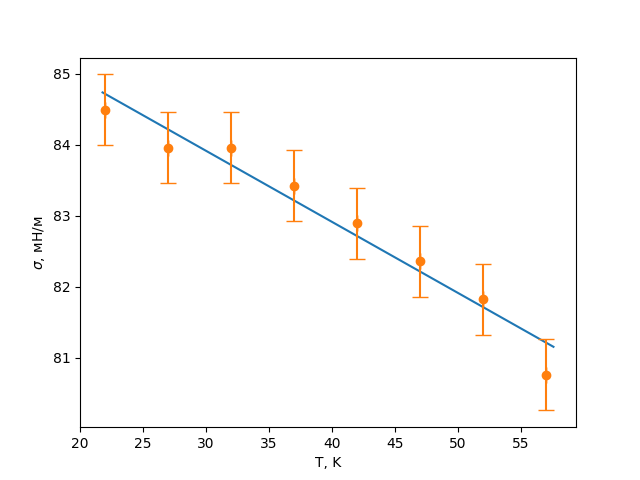
\includegraphics[scale=1.0]{sigma(t).png}
    \caption{График зависимости разницы давления от температуры}
\end{figure}

Из графика найдем: $(\frac{d\sigma}{dT} = -0.10 \pm 0.01)$ $ \text{мН/м} \cdot K$

Построим также $q(t)$ и $U_\text{п}/\text{П}(t)$

\begin{equation}
    q(T) = -T \frac{d\sigma}{dT}
\end{equation}
\begin{equation}
    U_\text{п}/\text{П}(T) = q(T) + \sigma(T)
\end{equation}

\begin{figure}[h!]
    \center
    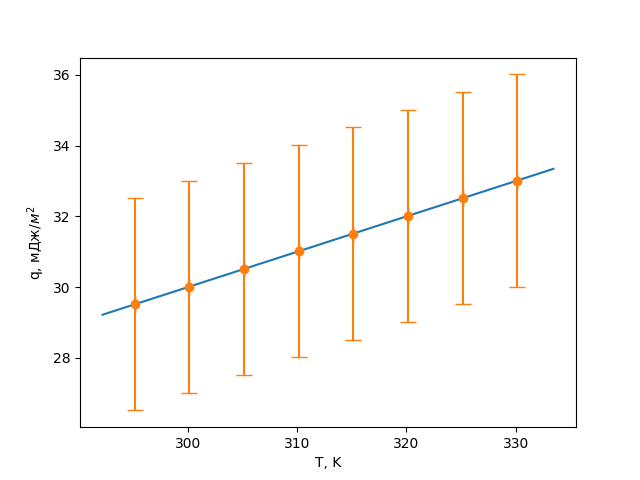
\includegraphics[scale=0.8]{q.png}
    \caption{График зависимости образования единицы поверхности жидкости от температуры}
\end{figure}

\begin{figure}[h!]
    \center
    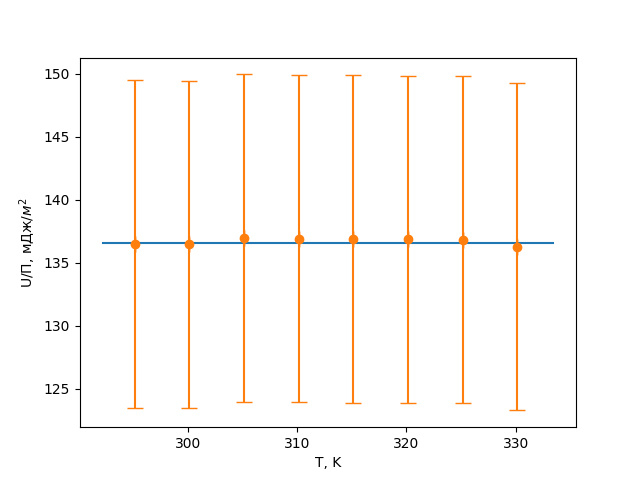
\includegraphics[scale=0.8]{U.png}
    \caption{График поверхностной энергии единицы площади от температуры}
\end{figure}

\section{Вывод}

Мы определили диаметр игры с точностью, сравнимой с микрометром.

Мы определили глубину погружения иглы с точностью линейки.

Мы построили график коэффициента поверхностного натяжения воды от температуры,
который, к сожалению, плохо совпал с табличными значениями.

Мы определили $\frac{d\sigma}{dT} = (-0.10 \pm 0.01)$ $ \text{мН/м} \cdot K$

Мы определили, что $U_\text{п}/\text{П} = (136 \pm 14)$ $ \text{мН/м} \cdot K$ 
и не зависит от температуры
\end{document}
